\newpage
\section{IMPACTO SOCIAL, ECONÓMICO Y MEDIOAMBIENTAL} \label{impacto}

A continuación, se detallan las contribuciones al desarrollo social, económico y medioambiental de la temática trabajada en el proyecto: los \acrlongpl{smr} y la simulación para la educación y formación nuclear. Para ello, se toman como referencia los Objetivos de Desarrollo Sostenible (ODS) y se explica el modo en el que se potencian algunos de ellos:

\begin{itemize}
    \item \textbf{Objetivo 1 - Fin de la pobreza:} La meta 4 de este ODS consiste en \textit{``garantizar que todos los hombres y mujeres, en particular los pobres y los más vulnerables, tengan los mismos derechos a los recursos económicos, así como acceso a los servicios básicos, la propiedad y el control de las tierras y otros bienes, la herencia, los recursos naturales, las nuevas tecnologías y los servicios económicos''} (\cite{ODS}).
    
    Tal y como se explica en el punto ...

    \item \textbf{Objetivo 4 - Educación de calidad:} La meta 4 de este ODS se propone \textit{``aumentar considerablemente el número de jóvenes y adultos que tienen las competencias necesarias, en particular técnicas y profesionales, para acceder al empleo, al trabajo decente y al emprendimiento''} (\cite{ODS}).
    
    Como se ha explicado en el apartado ...
\end{itemize}

\begin{figure}[h!]
    \centering
    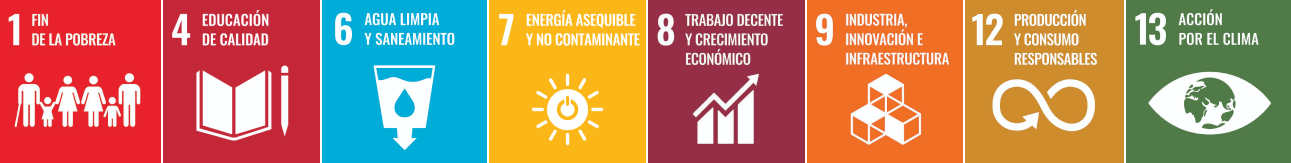
\includegraphics[width=\textwidth]{content/figures/ODS_TFG.png}
    \caption{Objetivos de Desarrollo Sostenible relacionados con este proyecto (\cite{ODS}).}
    \label{fig:ods_tfg}
  \end{figure}